\documentclass[11pt,a4paper]{article}
\usepackage[margin=25mm]{geometry}
\usepackage{graphicx}
\usepackage{enumitem}
\setlength{\parindent}{0pt}
\begin{document}

\section*{Setup}

\subsection*{Prerequisites}
\begin{itemize}[nosep]
  \item BioyondWorks, installed on the PC.
  \item The Bioyond Python package (a .whl file). Contact us or Bioyond to get it.
  \item Python 3.10 or newer.
  \item Run 	exttt{.	extbackslash install.ps1 -SdkWheel <path to the .whl file>}.
  \item Close BioyondWorks.
\end{itemize}

\subsection*{Hardware}
\begin{center}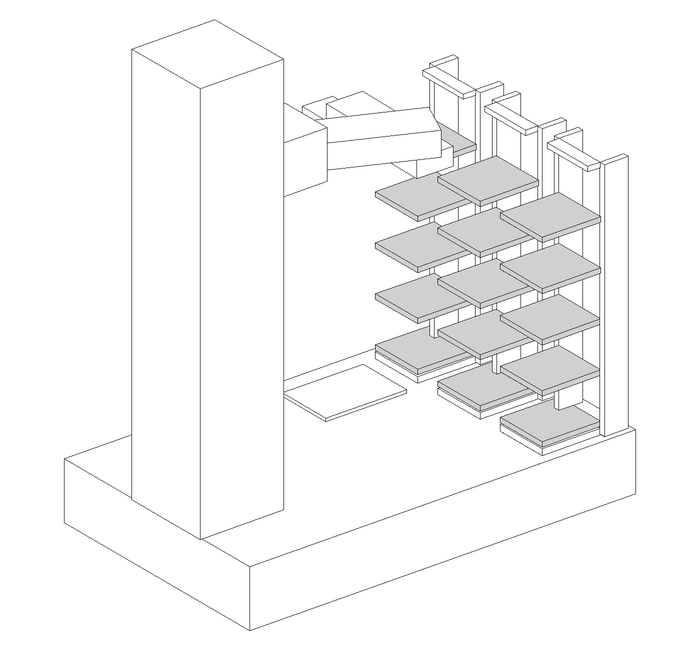
\includegraphics[width=0.6\textwidth]{img/cell_model.png}\end{center}
\begin{enumerate}[nosep]
  \item Connect the power cable and the emergency stop to the arm. Turn on the main switch at the back. Wait until the status light is steady.
  \item Connect the PC to port 1 of the controller with a network cable.
  \item Screw the hotel onto the platform. The slots face the arm.
  \item Load the plates into the hotel. Start at A1.
\end{enumerate}
\begin{center}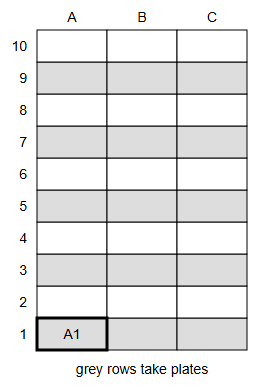
\includegraphics[width=0.35\textwidth]{img/hotel_matrix.png}\end{center}
\begin{enumerate}[nosep,resume]
  \item Place the ArUco plate on the rotation module.
\end{enumerate}

\subsection*{Setup}
\begin{enumerate}[nosep]
  \item Run \texttt{.\textbackslash install.ps1 -SdkWheel <path to the .whl file>}.
  \item Close BioyondWorks.
  \item Run \texttt{python cli.py setup}. The script ends with \texttt{READY}.
\end{enumerate}

\subsection*{Setup script in a nutshell}
\begin{itemize}[nosep]
  \item Upload some preset knowledge to the arm:
  \begin{itemize}[nosep]
    \item hotel slot positions
    \item rotation module seat position
    \item long-edge grip, short-edge grip, and grip torque probe procedure
    \item routes from each slot $\leftrightarrow$ rotation module
    \item slot-exit procedure
  \end{itemize}
  \item Calibrate cameras:
  \begin{itemize}[nosep]
    \item Run aruco intrinsic and extrinsic calibration
    \begin{itemize}[nosep]
      \item Upload to the camera box
    \end{itemize}
    \item optional test script
    \begin{itemize}[nosep]
      \item for each slot $\leftrightarrow$ rotation module
    \end{itemize}
  \end{itemize}
\end{itemize}

\end{document}
